\documentclass[11pt]{article}
\usepackage[textwidth=18.0cm, textheight=23.0cm, top=2.0cm]{geometry}
\usepackage{pst-all}
\usepackage{amssymb}
\usepackage{tikz}
\usepackage{underscore}\begin{document}
\pagestyle{empty}


ClassName: \underline{\textbf{Class_04.2bp-5}}
\par
BinSize: \underline{\textbf{100 × 100}}
\par
ReduceSize: \underline{\textbf{100 × 100}}
\par
TypeNum: \underline{\textbf{19}}
\par
Num: \underline{\textbf{20}}
\par
OutS: \underline{\textbf{10000}}
\par
InS: \underline{\textbf{7605}}
\par
Rate: \underline{\textbf{0.761}}
\par
UB: \underline{\textbf{1}}
\par
LB0: \underline{\textbf{1}}
\par
LB: \underline{\textbf{1}}
\par
LBWithCut: \underline{\textbf{1}}
\par
NodeCut: \underline{\textbf{0}}
\par
ExtendedNodeCnt: \underline{\textbf{1}}
\par
GenNodeCnt: \underline{\textbf{1}}
\par
PrimalNode: \underline{\textbf{0}}
\par
ColumnCount: \underline{\textbf{1}}
\par
TotalCutCount: \underline{\textbf{0}}
\par
RootCutCount: \underline{\textbf{0}}
\par
LPSolverCnt: \underline{\textbf{1}}
\par
PricingSolverCnt: \underline{\textbf{0}}
\par
BranchAndBoundNum: \underline{\textbf{1}}
\par
isOpt: \underline{\textbf{true}}
\par
TimeOnInitSolution: \underline{\textbf{600.000 s}}
\par
TimeOnPrimal: \underline{\textbf{0.000 s}}
\par
TimeOnPricing: \underline{\textbf{0.000 s}}
\par
TimeOnRmp: \underline{\textbf{0.063 s}}
\par
TotalTime: \underline{\textbf{600.344 s}}
\par
\newpage


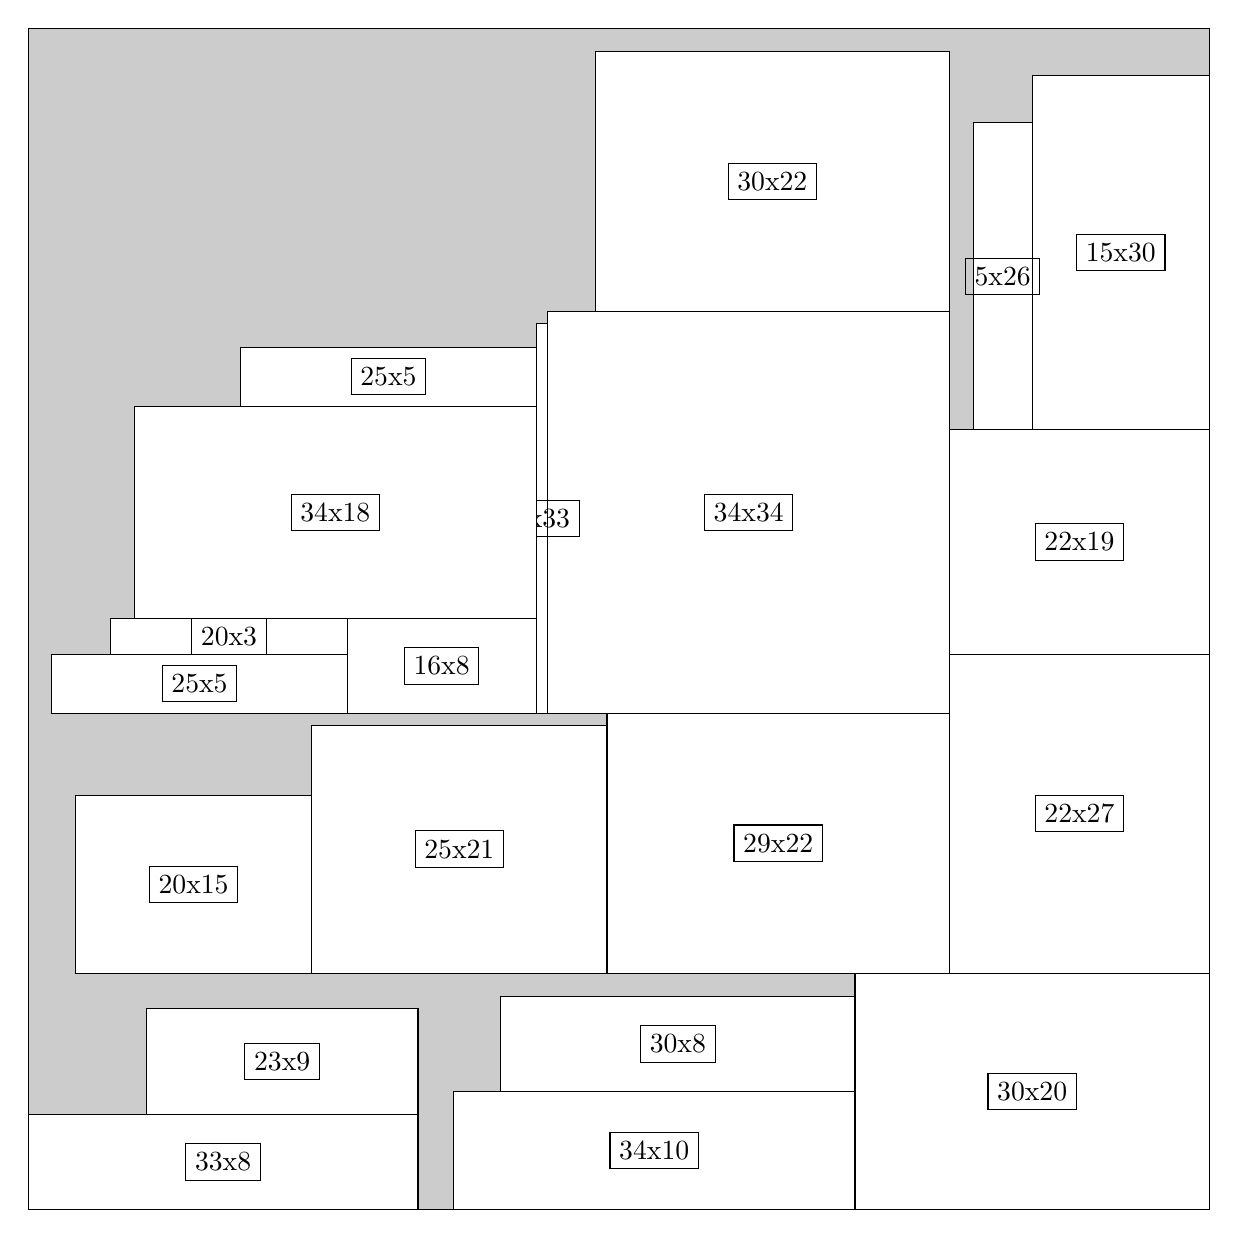
\begin{tikzpicture}[shorten >=1pt,scale=1.0,every node/.style={scale=1.0},->]
\tikzstyle{vertex}=[circle,fill=black!25,minimum size=14pt,inner sep=0pt]
\filldraw[fill=gray!40!white, draw=black] (0,0) rectangle (15.0,15.0);
\foreach \name/\x/\y/\w/\h in {30x20/10.5/0.0/4.5/3.0,34x10/5.3999999999999995/0.0/5.1/1.5,30x8/6.0/1.5/4.5/1.2,33x8/0.0/0.0/4.95/1.2,23x9/1.5/1.2/3.4499999999999997/1.3499999999999999,22x27/11.7/3.0/3.3/4.05,22x19/11.7/7.05/3.3/2.85,15x30/12.75/9.9/2.25/4.5,5x26/12.0/9.9/0.75/3.9,29x22/7.35/3.0/4.35/3.3,25x21/3.5999999999999996/3.0/3.75/3.15,20x15/0.6/3.0/3.0/2.25,34x34/6.6/6.3/5.1/5.1,30x22/7.199999999999999/11.4/4.5/3.3,1x33/6.45/6.3/0.15/4.95,16x8/4.05/6.3/2.4/1.2,25x5/0.3/6.3/3.75/0.75,20x3/1.05/7.05/3.0/0.44999999999999996,34x18/1.3499999999999999/7.5/5.1/2.6999999999999997,25x5/2.6999999999999997/10.2/3.75/0.75}
\filldraw[fill=white!40!white, draw=black] (\x,\y) rectangle node[draw] (\name) {\name} ++(\w,\h);
\end{tikzpicture}


w =30 , h =20 , x =70 , y =0 , v =600
\par
w =34 , h =10 , x =36 , y =0 , v =340
\par
w =30 , h =8 , x =40 , y =10 , v =240
\par
w =33 , h =8 , x =0 , y =0 , v =264
\par
w =23 , h =9 , x =10 , y =8 , v =207
\par
w =22 , h =27 , x =78 , y =20 , v =594
\par
w =22 , h =19 , x =78 , y =47 , v =418
\par
w =15 , h =30 , x =85 , y =66 , v =450
\par
w =5 , h =26 , x =80 , y =66 , v =130
\par
w =29 , h =22 , x =49 , y =20 , v =638
\par
w =25 , h =21 , x =24 , y =20 , v =525
\par
w =20 , h =15 , x =4 , y =20 , v =300
\par
w =34 , h =34 , x =44 , y =42 , v =1156
\par
w =30 , h =22 , x =48 , y =76 , v =660
\par
w =1 , h =33 , x =43 , y =42 , v =33
\par
w =16 , h =8 , x =27 , y =42 , v =128
\par
w =25 , h =5 , x =2 , y =42 , v =125
\par
w =20 , h =3 , x =7 , y =47 , v =60
\par
w =34 , h =18 , x =9 , y =50 , v =612
\par
w =25 , h =5 , x =18 , y =68 , v =125
\par
\newpage


\end{document}